\chapter{Prototyping in [Case]}

\section{System description}
The setup consists of a Linux server (preferable af Debian distribution) running on a server. The setup could run on any PC acting as server, but it is essential that the client knows what nameserver to contact first, when going for a root server. Instead of asking the nameserver providede by most ISP's, it should use the bind server running on the network.

Most modern mid-end routers has the ability to do some basic DNS forwarding. In our case this feature would be very useful, to forward any DNS requests to the BIND9 server on the network, instead of going directly to the one provided by the ISP. Mostly, the default setup could look something like this:

\begin{center}
	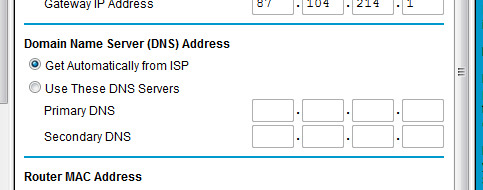
\includegraphics[scale=1.0]{router_DNS.png}
	\captionof{figure}{DNS Nameserver forwarding on NETGEAR router}
\end{center}

From here on, our local nameserver will handle any DNS lookup on the network, allowing us to filter, cache and forward all trafic, as needed.

\section{BIND DNS server}
The most popular version of the BIND DNS server, is version nine, also calle BIND9. This can be downloaded from the debian public repositories using aptitude. Install BIND9 using the following command:

\begin{center}
	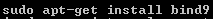
\includegraphics[scale=1.0]{apt-get_bind9.png}
%	\captionof{figure}{DNS Nameserver forwarding on NETGEAR router}
\end{center}

\section{Setup of BIND server}
First we set up BIND as a caching nameserver. We added localhost, 127.0.0.1, as the first nameserver in "/etc/resolvconf/resolv.conf.d/head". Then we set set up a DNS forwarder to take care of all the non cached results by adding its IP address to "/etc/bind/named.conf.options". After these steps was the only thing left to do to restart the bind server and the then we had blazing fast DNS lookups.


\subsection{Choose DNS server to forward to}
To find the most optimal DNS server to forward to, we chose to use Googles Namebench to decide for us. It runs a full fledged test suite that tests all available DNS servers for which has the fastest response times.  

\section{Tests}
After setting up BIND to act as a forwarding DNS server, we must test to see if it actually worked!

To test this, we will use the \textit{dig} tool, to check that the forwarding works, and that caching has a noticeable effect on the DNS look up times. 
\subsection{dig tool}
To test DNS look up times, the Domain Information Groper is invoked in the command line.

This will give us the query time and the forwarding server, used in the query where

\textbf{Query time}
Denotes the time (in ms) it took to resolve the name into an IP address.
This query time should go down considerably on repeated attempts as a result of caching DNS resolutions.

and

\textbf{SERVER}
Denotes the DNS forwarding server used. This should be the address of the BIND server (127.0.0.1, as the BIND server is checking on the localhost interface).


\subsection{Testing}
\textbf{Forwarding}

In this test, dig is invoked to resolve the website www.svejstrup.org. 
The picture is part of the output of the dig tool and shows the address used as DNS server.

\begin{center}
	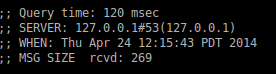
\includegraphics[scale=1.0]{ForwardingSmall.png}
%	\captionof{figure}{DNS Nameserver forwarding on NETGEAR router}
\end{center}

\textbf{Caching}

In this test, dig is invoked to resolve the website www.svejstrup.org.
The picture is the full output of dig and shows the query time \textit{the first time} dig is invoked to do the resolving. This should give an idea of the resolving time \textit{before} the DNS is cached.

\begin{center}
	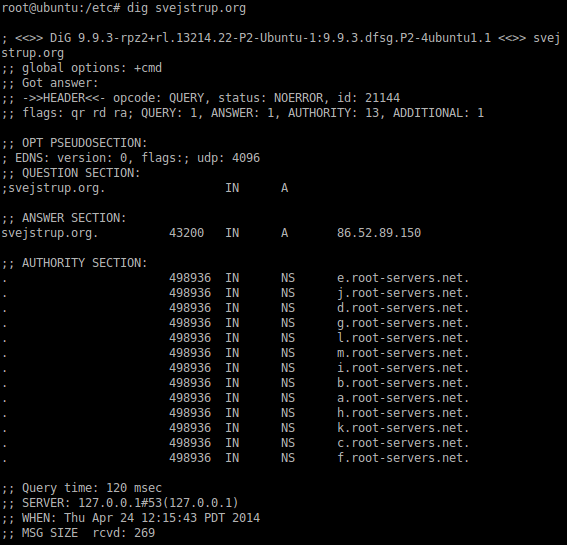
\includegraphics[scale=1.0]{DigFullBeforeCaching.png}
%	\captionof{figure}{DNS Nameserver forwarding on NETGEAR router}
\end{center}

After the initial run of dig, the DNS resolve should now be cached in the BIND server. To test this, we run dig again on the same website shortly after the first run:

\begin{center}
	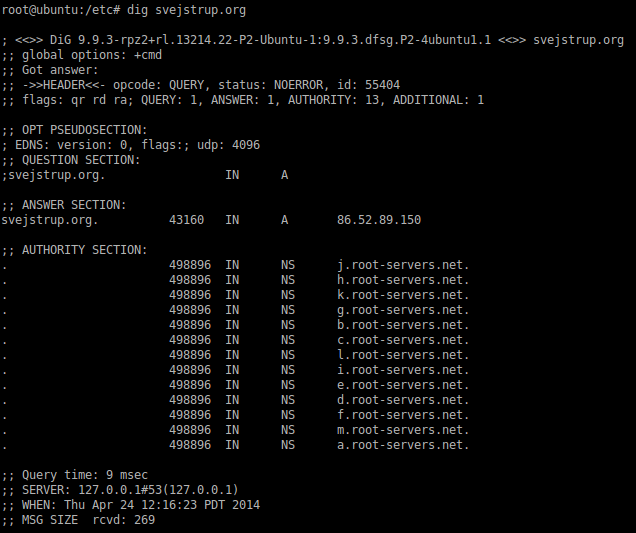
\includegraphics[scale=1.0]{DigFull.png}
%	\captionof{figure}{DNS Nameserver forwarding on NETGEAR router}
\end{center}

\textbf{IP address}
of the server is also seen in the dig printout (86.52.89.150).

\section{Results}
\subsection{Forwarding}
The DNS server used for DNS resolution is now 127.0.0.1,the address of localhost which BIND listens on.

\subsection{Caching}
We see that, before caching the query time was \textit{120 ms} and after the caching it was all the way down to \textit{9 ms}.

So that is a decrease of 111 ms, a sizeable decrease.



%This chapter should contain an in-depth description of prototyping
%with the technology, i.e. DNS, DDS, or RMI. That is, you analyze,
%design, implement, and test
%\begin{itemize}
%\item a very limited, but functional prototype that utilizes the
%  technology under consideration.
%\end{itemize}

%You define your own prototype and the context in which it should
%function; the list below is for your inspiration.

%\begin{itemize}
%\item Domain Name System: A public school or a medium sized company
%  would like to host their own DNS and/or forward requests to OpenDNS.
%\item Data Distribution Service: A hospital or a production factory
%  would like to employ Connext DDS to distribute mission critical
%  data.
%\item Java Remote Method Invocation: A company is setting up
% facilities, e.g. parcel or luggage sorters, abroad and would like to
%  be able to access back-end methods and data at home.
%\end{itemize}

%In your analysis you should at least address and/or include

%\begin{itemize}
%\item Overall diagram and description of the prototype
%\item Relevance of the technology under consideration to your prototype
%item How the technology is included in your prototype
%\item Definition of a small set of realistic use-cases and related
%  functional requirements
%\end{itemize}

%The design, implementation, and test should at least address and/or include:

%\begin{itemize}
%\item Diagrams, e.g. UML, supplemented with code snippets of most important parts
%\item Test and evaluation of your system: Does it work as intended?
%\item Evaluation of the prototype and the technology employment as a
%  whole
%\end{itemize}